\documentclass[conference]{IEEEtran}
\IEEEoverridecommandlockouts
\usepackage{cite}
\usepackage{amsmath,amssymb,amsfonts}
\usepackage{graphicx}
\usepackage{booktabs}
\usepackage{textcomp}
\usepackage{xcolor}
\usepackage{url}
\graphicspath{{figures/}}
\setlength{\tabcolsep}{3.5pt}
\def\BibTeX{{\rm B\kern-.05em{\sc i\kern-.025em b}\kern-.08em T\kern-.1667em\lower.7ex\hbox{E}\kern-.125emX}}

\begin{document}

\title{FidelityMem: Recall-Constrained Adaptive Hybrid Memory for LLM Agents}

\author{\IEEEauthorblockN{Vaibhav Bansal}
\IEEEauthorblockA{\textit{Independent researcher}\\
vaibhav.bansal2020@gmail.com}}

\maketitle

\begin{abstract}
Long-running LLM agents accumulate more history than fits in a context window, and the memory systems that compress and retrieve that history expose no bound on the evidence they lose. We present FidelityMem, a memory layer whose control variable is a recall-retention bound: minimise storage, context tokens and latency subject to the compressed index retaining at least $\rho$ of the recall of the best raw retrieval available. The bound is enforced twice. At admission, a deterministic fidelity gate builds entity, number, date and negation probes from the raw source and backs the compressor off level by level until the compressed form satisfies them. At policy time, a guarded controller searches over compression level, route pool, dense-route weight, expansion budget and gate profile, confirms the cheapest feasible configuration on a held-out split of a query log, and keeps the previous policy for rollback. On a consistent-world synthetic benchmark from 300 to 10\,000 records, FidelityMem reaches 0.995--1.000 Recall@10 at 41--48\% of raw storage against eleven baselines, including architecture-faithful re-implementations of Mem0, Letta, Zep, A-MEM and HippoRAG. On LoCoMo, BM25 is the strongest retriever (Recall@10 0.914) because the benchmark's questions reuse the evidence's words; the controller detects this from the query log and ties it (0.913). When the questions are paraphrased, BM25 loses 28 points and lexical--dense fusion 19. Calibrated on each regime's query log alone, the controller selects lexical-only retrieval on literal queries and lexical+dense on paraphrased queries, landing within 0.7 points of the best fixed configuration in every regime, which no fixed configuration does. With a Claude reader and judge on 200 LoCoMo questions, answer accuracy matches BM25 at 21\% lower cost when an LLM compressor is used under the gate.
\end{abstract}

\begin{IEEEkeywords}
agent memory, retrieval-augmented generation, hybrid retrieval, lossy compression, reciprocal-rank fusion, recall constraint, LLM agents
\end{IEEEkeywords}

\section{Introduction}
Agent memory research has converged on one architecture: a short working context, typed long-term stores, compression, and retrieval that fuses lexical, dense and graph signals. MemGPT introduced hierarchical context management \cite{memgpt}; HippoRAG added entity graphs and personalised PageRank \cite{hipporag}; Zep/Graphiti a bi-temporal knowledge graph \cite{zep}; Mem0 reduced memory to atomic LLM-extracted facts \cite{mem0}; A-MEM linked notes by similarity \cite{amem}. The components are no longer novel individually.

What remains unsolved is \emph{control}. Every system above decides how much to compress and how to retrieve with fixed heuristics or with learning aimed at answer accuracy. None states a recall bound and enforces it. The documented consequence is silent evidence loss: a $36.7\times$ compression of structured facts left 60\% irrecoverable \cite{facts}; summarisers drop qualifiers \cite{fidelity}; rewrites launder hedged hearsay into asserted fact \cite{factwash}. Retrieval metrics do not catch this, because the right memory id is retrieved while the fact inside it is gone.

A second unsolved problem is the choice of retrieval regime. Our measurements on LoCoMo show that BM25 beats every hybrid when questions reuse the evidence's words, and that the ordering reverses once questions are paraphrased. No fixed configuration is right for both, and a 2026 study found no lightweight adaptive router that beat a fixed sparse--dense blend under cross-validation \cite{fairness}.

FidelityMem's contribution is a recall-constrained controller with an enforceable gate, and a protocol that measures whether the bound holds. We claim:
\begin{enumerate}
\item A deterministic fidelity gate, built from the raw source, prevents fact loss at admission without an LLM and without labels (Sec.~\ref{sec:gate}).
\item A guarded search over discrete compression levels, route pools, dense-route weights and expansion budgets finds the cheapest policy that holds a retention bound $\rho$ and confirms it out of sample (Sec.~\ref{sec:controller}).
\item Relation chaining after fusion recovers the second hop of two-hop questions that reciprocal-rank fusion buries (Sec.~\ref{sec:retrieval}, ablation in Sec.~\ref{sec:ablation}).
\item On a controlled synthetic protocol with shared components, the design dominates six current memory architectures on recall, complete-set recall and stored tokens at every scale tested (Sec.~\ref{sec:synthetic}). On LoCoMo it ties the strongest baseline, BM25, and we show why (Sec.~\ref{sec:paraphrase}).
\item The controller selects the retrieval regime from the query log alone, lexical-only when queries are literal and lexical+dense when they are paraphrased, matching the best fixed configuration in each regime out of sample (Sec.~\ref{sec:regime}). To our knowledge this is the first positive result for a query-log-adaptive sparse--dense selector in agent memory.
\end{enumerate}
Code, benchmark generator, evaluation stack and all result files are released as the \texttt{fidelitymem} Python package.

\section{Related Work}
FidelityMem reuses the stores and retrieval signals of current systems and differs in what controls them. Table~\ref{tab:related} places it against the nearest work on three axes: memory architectures, compression fidelity, and adaptive hybrid retrieval. The negative result of \cite{fairness}, that oracle tuning of the sparse--dense weight has 22\% headroom which no lightweight adaptive router realised under cross-validation, is the contrast for Sec.~\ref{sec:regime}: our selector is a discrete guarded search with an out-of-sample confirmation step, not a per-query predictor.

\begin{table*}[t]
\caption{Nearest work and the difference}
\label{tab:related}
\centering
\footnotesize
\begin{tabular}{p{3.1cm}p{4.2cm}p{3.6cm}p{5.6cm}}
\toprule
System & Core mechanism & FidelityMem takes & FidelityMem adds \\
\midrule
MemGPT / Letta \cite{memgpt} & Core, recall and archival tiers paged by the agent & Working vs long-term split & Retention-scored window with boundary triggers; no agent in the loop \\
HippoRAG \cite{hipporag} & OpenIE entity graph, personalised PageRank from query entities & Graph seeded by query entities & Relation-following with hub penalty; relation chaining after fusion \\
Zep / Graphiti \cite{zep} & Bi-temporal entity graph, hybrid search, edge invalidation & Temporal validity, supersede-not-delete & Contradictions limited to exclusive predicates; fidelity gate \\
Mem0 \cite{mem0} & LLM-extracted atomic facts, vector search & Fact-level dedupe & Raw evidence retained and expandable; LLM-free ingestion \\
A-MEM \cite{amem} & Notes linked to nearest neighbours & Linked expansion & Explicit relations instead of similarity links \\
R$^3$Mem \cite{r3mem} & Reversible compression via virtual memory tokens & Reversibility as a requirement & Reversibility by immutable raw pointer \\
EvolveMem \cite{evolvemem}, MemRL \cite{memrl} & Learned retrieval configuration or utility & Feedback-driven utility & Constraint-based optimisation, hold-out gate, rollback \\
CrystalMem \cite{crystalmem} & Four fidelity states under a byte budget & Fidelity as an explicit state & Bound on measured recall rather than bytes \\
ARC \cite{arc} & Old observations replaced by addressable citations & Raw source always addressable & Compression only when the gate certifies it \\
MemRefine \cite{memrefine}, rate--distortion view \cite{ratedist} & Compression under a hard budget & The budget--fidelity trade-off & Recall floor instead of a budget; out-of-sample confirmation \\
Lexical--dense fusion for conversational memory \cite{tfusion}, adaptive WRRF \cite{wrrf}, vstash \cite{vstash} & Hybrid retrieval with fixed or per-query fusion weights & Weighted RRF over lexical and dense routes & Weight chosen by the controller from the query log under the recall bound, with the compression level \\
Facts as objects \cite{facts}, Fidelity before structure \cite{fidelity}, FACTWASH \cite{factwash} & Evidence that gist compression loses facts & Motivation and probe design & A gate that enforces it per memory \\
\bottomrule
\end{tabular}
\end{table*}

\section{Method}
\begin{figure*}[t]
\centering
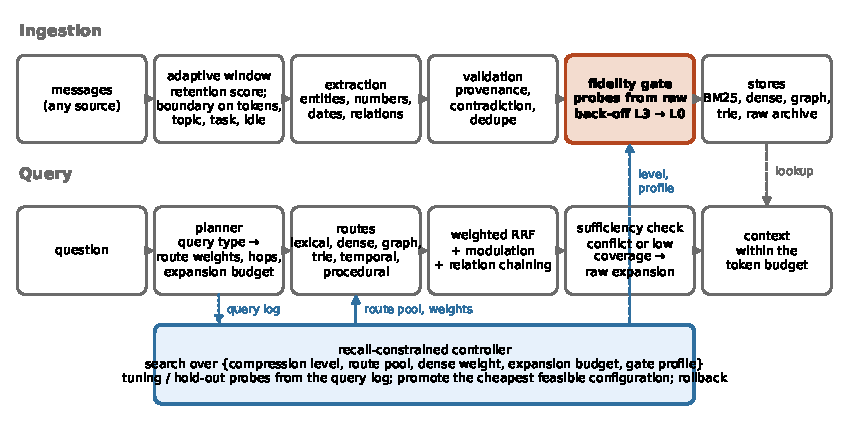
\includegraphics[width=\textwidth]{fig_architecture.pdf}
\caption{FidelityMem workflow. Top: ingestion through the adaptive window, extraction, validation and the fidelity gate into the stores. Bottom: a query through the planner, the routes, weighted RRF with modulation and relation chaining, the sufficiency check and the token budget. The controller sets the route pool and weights on the query side and the compression level and gate profile on the ingestion side, from the query log.}
\label{fig:arch}
\end{figure*}

\subsection{Data model and admission}
An \emph{episode} is immutable raw text with provenance (source, type, tenant, timestamp, trust, authority). A \emph{memory} is a derived, searchable record pointing at exactly one episode: compressed text, compression level, extracted entities, numbers, dates, negated sentences, relations, types (semantic, episodic, procedural, relational), confidence, validity interval, utility and a fidelity score. Memories are superseded, never deleted; user-requested forgetting removes memory and episode together.

Messages enter an adaptive working window scored by retention $R(m) = w_s S_{\mathrm{sem}} + w_r S_{\mathrm{rec}} + w_i S_{\mathrm{imp}} + w_t S_{\mathrm{task}} + w_c S_{\mathrm{conf}} + w_u S_{\mathrm{util}}$, with task continuity weighted highest. Boundaries fire on token pressure, topic shift, task completion and inactivity; each boundary hands its segment to extraction. Admission runs three stages: provenance and contradiction detection with supersede-not-delete and demotion of instructions found in untrusted content; durability scoring and near-duplicate removal; and the fidelity gate.

\subsection{Reversible compression and the fidelity gate}
\label{sec:gate}
Compression is a four-level ladder: L0 raw; L1 extractive at about 60\% of sentences by salience; L2 key facts, keeping only sentences carrying an entity, number, date or negation; L3 gist, one salient sentence. An LLM compressor plugs in through a one-method protocol and is gated identically.

From the \emph{raw} text we build a probe set: one probe per entity (weight 1), number (1.5), date (1.5) and negated sentence (2, satisfied only if at least 60\% of its content words and a negation cue survive). The \emph{content} profile adds up to 16 salient content-word probes (0.5). The gate accepts level $\ell$ iff the weighted probe score is at least $\rho$; otherwise it backs off to $\ell-1$, and L0 always passes. Because probes come from the source rather than the summary, the gate measures what was lost. The probe set is stored with the memory so recompression under a new policy reuses it.

\subsection{Query-aware hybrid retrieval}
\label{sec:retrieval}
The planner classifies a query as factual, temporal, multi-hop, exact, procedural or code-review and sets route weights, graph hops, expansion budget and whether raw expansion is mandatory. The controller's route pool is authoritative: the planner may weight routes but never adds one the controller excluded. Routes: BM25 ($k_1 = 1.5$, $b = 0.75$); dense (any embedder; MiniLM-L6 over overlapping 120-word windows in the experiments below); relation graph with relation-following before co-mention, a hub penalty and no traversal through hub entities (degree above 40); a trie over identifier-like tokens and 2--4-gram phrases; temporal and procedural routes restricted by memory type.

Route results are fused by weighted reciprocal-rank fusion, $s(d) = \sum_r w_r/(60 + \mathrm{rank}_r(d))$, then multiplied by $1 + 0.05\,\mathrm{recency} + 0.2\tanh(\mathrm{utility}) + 0.05\,\mathrm{authority} + \mathrm{type\ boost}$, which is small by design so that it breaks ties without outranking a clearly better match. Two steps follow that the baselines lack. \emph{Relation chaining}: if a top result states $A \xrightarrow{p} B$ with $A$ named in the query, memories in which $B$ is a relation subject are promoted beside it, recovering the second hop that rank fusion buries. \emph{Sufficiency and expansion}: a memory is expanded to its raw episode, within a budget, when the task is exact, confidence or fidelity is low, retrieved memories conflict on an exclusive predicate, or the query's content words are barely covered by the compressed text. Context is trimmed to the token budget, falling back from raw to compressed before dropping.

\subsection{Recall-constrained controller}
\label{sec:controller}
\begin{figure}[t]
\centering
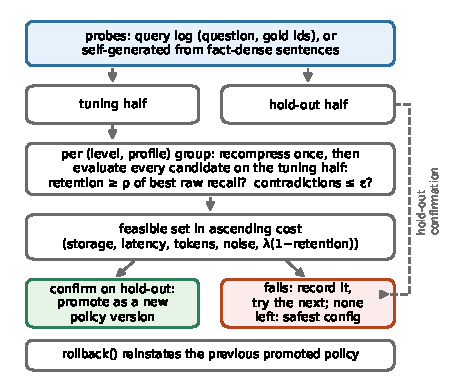
\includegraphics[width=\columnwidth]{fig_controller.pdf}
\caption{The controller's guarded search. Candidates are evaluated on the tuning half, walked in ascending cost, and promoted only after confirming on the hold-out half.}
\label{fig:ctrl}
\end{figure}
A configuration $\pi$ is a compression level in $\{0,1,2,3\}$, a top-$k$, an expansion budget in $\{0,2\}$, a route pool from five sets, a gate profile in \{facts, content\} and a dense-route weight in $\{0.5, 1.0\}$. The controller minimises
\begin{equation}
\begin{split}
\mathrm{cost}(\pi) = \; & \alpha\,\mathrm{StorageRatio} + \beta\,\mathrm{Latency} + \gamma\,\mathrm{TokensPerQuery} \\
& + \delta\,\mathrm{Noise} + \lambda\,(1 - \mathrm{Retention}(\pi))
\end{split}
\end{equation}
subject to $\mathrm{Retention}(\pi) = \mathrm{Recall}_\pi@K / \mathrm{Recall}_{\mathrm{rawbest}}@K \ge \rho$ and $\mathrm{UnresolvedContradictionRate} \le \varepsilon$, where $\mathrm{Recall}_{\mathrm{rawbest}}$ is the best raw (L0) retrieval over all route pools, so the reference is not the candidate's own uncompressed twin.

Retention is measured on probe queries: either self-generated (the most fact-dense sentence of a sampled episode with a third of its words dropped) or a query log of (question, gold episode) pairs. Probes are split into tuning and hold-out halves (Fig.~\ref{fig:ctrl}). Every candidate is evaluated on the tuning half, grouped by level and profile so the store is recompressed once per group; feasible candidates are walked in ascending cost and confirmed on the hold-out half; the first that confirms is promoted as a new policy version. If none confirms, the safest configuration is promoted. Rejected candidates stay in the history for audit and rollback reinstates the previous promoted policy.

\section{Experimental Protocol}
\textbf{Synthetic benchmark.} A seeded generator produces a consistent world of 200 services, each with one database, owner and dependency, so no gold fact is legitimately contradicted. Every episode is a fact sentence embedded in 2--4 sentences of workplace filler. Question families: factual, temporal, two-hop (two gold episodes) and exact-value (two numbers and a negated constraint). Distractors fill to the record count, 30\% hard (same names, no decision) and 70\% off-topic. Record counts 300, 1\,000, 3\,000 and 10\,000; $K=10$; three seeds, each a different world.

\textbf{Real data.} LoCoMo \cite{locomo}: 10 multi-session conversations, 5\,882 turns, 1\,986 questions with evidence dialogue ids as retrieval ground truth; categories multi-hop, temporal, open-domain, single-hop and adversarial (no gold, excluded from recall). One memory per session (272 sessions). Per seed, 30\% of questions are held out as the controller's query log and never scored.

\textbf{Paraphrase regimes.} Every question is rewritten with WordNet synonyms (first lemma of a different stem; names, numbers, dates and stop words protected) at two strengths: 45\% and 91\% of eligible content words replaced.

\textbf{Metrics.} Recall@$K$ against gold episode ids, complete-evidence-set recall, MRR, nDCG@$K$, tokens served per query, p50/p95 retrieval latency, stored tokens, raw-expansion rate, and retention against the best raw retrieval. Means over three seeds with 95\% $t$-intervals; bootstrap over questions for single-seed runs.

\textbf{Baselines.} Classic: fixed window, BM25, dense, BM25+dense RRF, lossy L3 summary + BM25. Architecture-faithful re-implementations sharing the same extractors, BM25 and embedder: window+trie, MemGPT-style, Mem0-style, Zep-style, A-MEM-style, HippoRAG-style. These are not vendor code; the vendors require an LLM to ingest, which would confound architecture with model.

\textbf{Embedder.} All dense routes in every system share one embedder: spaCy word vectors in the original runs, all-MiniLM-L6-v2 (ONNX, CPU) in the runs reported here, long records embedded as the mean of overlapping 120-word windows.

\textbf{LLM evaluation.} A Claude Opus 5.5 reader (low effort) answers from the served context only and abstains when it lacks the answer; a Claude Sonnet 5.5 judge marks the answer against the gold. 200 test questions, seed 0.

\section{Results}
\subsection{Synthetic benchmark at four scales}
\label{sec:synthetic}
\begin{figure}[t]
\centering
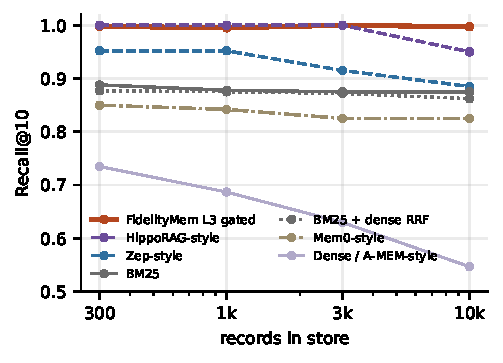
\includegraphics[width=\columnwidth]{fig_scale.pdf}
\caption{Recall@10 against store size (3 seeds). FidelityMem at level 3 holds 0.995--1.000 while storing 44\% of the raw tokens; graph-first architectures fall at 10\,000 records; BM25 never reaches the second hop.}
\label{fig:scale}
\end{figure}
FidelityMem holds 0.995--1.000 Recall@10 and complete-set recall from 300 to 10\,000 records while the controller stores 41--48\% of the raw tokens (Fig.~\ref{fig:scale}, Table~\ref{tab:synthetic}). HippoRAG-style ties it to 3\,000 records at full storage and falls to 0.950 at 10\,000, where hub entities dilute two-hop spreading; Zep-style falls from 0.952 to 0.885; BM25 stays at 0.875--0.888 and never reaches the second hop (complete-set recall 0.75 at every scale). With no access to the questions the controller selected level 3 (one seed level 1) with the facts profile at every scale, at measured retention 0.98--1.00.

\begin{table}[t]
\caption{Recall@10 by record count (3 seeds, word-vector embedder)}
\label{tab:synthetic}
\centering
\scriptsize
\resizebox{\columnwidth}{!}{%
\begin{tabular}{lrrrrr}
\toprule
System & 300 & 1\,000 & 3\,000 & 10\,000 & Storage \\
\midrule
BM25 & 0.888 & 0.878 & 0.875 & 0.875 & 100\% \\
BM25 + dense RRF & 0.877 & 0.875 & 0.872 & 0.862 & 100\% \\
Lossy L3 summary + BM25 & 0.855 & 0.853 & 0.850 & 0.857 & 27\% \\
Window + trie & 0.875 & 0.875 & 0.875 & 0.875 & 100\% \\
MemGPT-style & 0.705 & 0.658 & 0.605 & 0.528 & 100\% \\
Mem0-style & 0.850 & 0.842 & 0.825 & 0.825 & 23\% \\
Zep-style & 0.952 & 0.952 & 0.915 & 0.885 & 100\% \\
A-MEM-style & 0.735 & 0.687 & 0.630 & 0.547 & 100\% \\
HippoRAG-style & 1.000 & 1.000 & 1.000 & 0.950 & 100\% \\
FidelityMem raw (L0) & 0.998 & 0.995 & 1.000 & 0.997 & 100\% \\
FidelityMem L3 gated & 0.998 & 0.995 & 1.000 & 0.997 & 44\% \\
FidelityMem controller & 0.998 & 0.995 & 0.977 & 0.997 & 41--48\% \\
\bottomrule
\end{tabular}}
\end{table}

\subsection{LoCoMo sessions with a sentence embedder}
\label{sec:locomo}
On real conversation BM25 is the strongest retriever and every fused configuration is below it (Table~\ref{tab:locomo}). The query-log controller selects lexical-only retrieval on every seed and ties BM25 (0.913 vs 0.914). The self-probe controller is not reliable here: on one of three seeds it accepted level-2 facts-profile compression that satisfied its self-generated fact probes while losing 22 points on real questions, because LoCoMo asks about activities and opinions that the facts profile discards. This is the case for calibrating on a query log. Compression at $\rho = 0.95$ is small on chat: the content-profile gate backs off to raw on almost every session (98\% storage), since a session carries a fact in nearly every sentence.

Fixed route weights do not change the picture: lexical 1.2 + dense 0.5 gives 0.907, lexical 1.2 + dense 1.0 gives 0.904, adding an identifier trie 0.903, a semantic-codebook trie 0.900, the graph route 0.882, all routes with planner weights 0.873. Every route added to BM25 lowers recall on this dataset in proportion to its weight.

\begin{table}[t]
\caption{LoCoMo sessions, Recall@10, MiniLM-L6 embedder, 3 seeds ($\pm$ 95\% CI)}
\label{tab:locomo}
\centering
\scriptsize
\resizebox{\columnwidth}{!}{%
\begin{tabular}{lrrrrr}
\toprule
System & R@10 & CR@10 & MRR & Storage & p95 ms \\
\midrule
BM25 & 0.914 $\pm$.016 & 0.876 & 0.770 & 100\% & 0.3 \\
Dense (MiniLM) & 0.751 $\pm$.008 & 0.711 & 0.467 & 100\% & 5.2 \\
BM25 + dense RRF & 0.899 $\pm$.012 & 0.855 & 0.658 & 100\% & 5.6 \\
Zep-style & 0.882 $\pm$.024 & 0.841 & 0.597 & 100\% & 7.2 \\
HippoRAG-style & 0.700 $\pm$.019 & 0.656 & 0.396 & 100\% & 7.6 \\
FM raw, all routes & 0.811 $\pm$.032 & 0.768 & 0.412 & 100\% & 9.6 \\
FM L3 gated, facts & 0.668 $\pm$.030 & 0.625 & 0.327 & 22\% & 3.7 \\
FM L3 gated, content & 0.804 $\pm$.029 & 0.760 & 0.410 & 98\% & 3.8 \\
FM controller, query log & \textbf{0.913} $\pm$.014 & 0.874 & 0.736 & 98\% & 1.3 \\
FM controller, self-probes & 0.838 $\pm$.313 & 0.798 & 0.648 & 73\% & 1.3 \\
\bottomrule
\end{tabular}}
\end{table}

\subsection{Why BM25 wins on LoCoMo: paraphrase robustness}
\label{sec:paraphrase}
\begin{figure}[t]
\centering
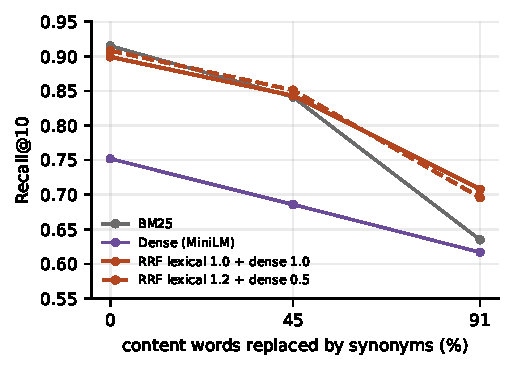
\includegraphics[width=\columnwidth]{fig_paraphrase.pdf}
\caption{Recall@10 as LoCoMo questions are rewritten with synonyms. BM25's lead is a property of literal questions; fusion overtakes it once wording drifts.}
\label{fig:para}
\end{figure}
BM25 matches stemmed surface forms only. Its lead is a property of how LoCoMo's questions were written: annotators reused the evidence's words. Rewriting the questions with synonyms reverses the ordering (Fig.~\ref{fig:para}, Table~\ref{tab:para}). Fusion is one point behind BM25 on literal questions, one point ahead at 45\% replacement and seven points ahead at 91\%, and the best dense weight rises as the wording drifts. The dense route alone loses only 13.5 points at full replacement against BM25's 28.

\begin{table}[t]
\caption{Recall@10 on original and paraphrased LoCoMo questions (1\,982 questions, seed 0; change in parentheses)}
\label{tab:para}
\centering
\scriptsize
\resizebox{\columnwidth}{!}{%
\begin{tabular}{lrrr}
\toprule
System & Original & 45\% replaced & 91\% replaced \\
\midrule
BM25 & 0.915 & 0.841 ($-$7.4) & 0.635 ($-$28.0) \\
Dense (MiniLM) & 0.752 & 0.686 ($-$6.6) & 0.617 ($-$13.5) \\
RRF lex 1.0 + dense 1.0 & 0.899 & 0.843 ($-$5.6) & \textbf{0.708} ($-$19.1) \\
RRF lex 1.2 + dense 1.0 & 0.903 & 0.843 ($-$6.0) & 0.697 ($-$20.5) \\
RRF lex 1.2 + dense 0.5 & 0.908 & \textbf{0.851} ($-$5.7) & 0.696 ($-$21.2) \\
\bottomrule
\end{tabular}}
\end{table}

\subsection{The controller selects the regime from the query log}
\label{sec:regime}
\begin{figure}[t]
\centering
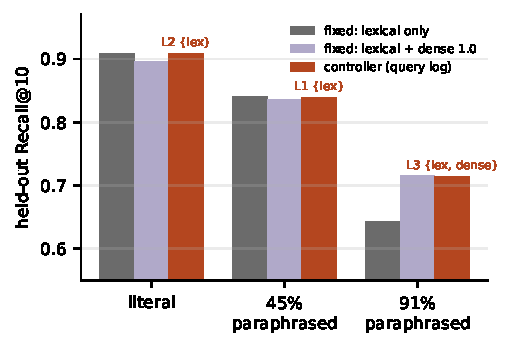
\includegraphics[width=\columnwidth]{fig_regime.pdf}
\caption{Held-out Recall@10 per query regime. The controller, calibrated on that regime's query log only, matches the best fixed configuration in each regime; neither fixed configuration does.}
\label{fig:regime}
\end{figure}
No fixed configuration is right for both regimes, so we ran the controller three times on the same store, calibrated on a 30\% split of the literal, the 45\%-paraphrased and the 91\%-paraphrased questions respectively (594 probes each) and scored on the other 70\% of the same regime, with fixed configurations scored on the same held-out split (Fig.~\ref{fig:regime}, Table~\ref{tab:regime}). The controller never sees the test questions. From the query log alone it switches from lexical-only to lexical+dense exactly where that switch pays, lands within 0.7 points of the best fixed configuration in every regime, and chooses a compression level in the same search. Lexical-only loses seven points on paraphrased queries; lexical+dense loses one point on literal queries; the controller loses neither. In the middle regime it accepts a 0.7-point loss for lexical-only's lower latency, which is the cost objective working inside the $\rho$ slack, and is stated as such.

\begin{table}[t]
\caption{Held-out Recall@10 per query regime (seed 0)}
\label{tab:regime}
\centering
\scriptsize
\resizebox{\columnwidth}{!}{%
\begin{tabular}{llrrr}
\toprule
Regime & Controller chose & Ctrl & Best fixed & Lexical \\
\midrule
Literal & L2, \{lex\} & \textbf{0.908} & 0.908 (lex) & 0.908 \\
45\% paraphr. & L1, \{lex\} & 0.839 & 0.846 (lex+d 0.5) & 0.841 \\
91\% paraphr. & L3, \{lex, dense\} & \textbf{0.714} & 0.716 (lex+d 1.0) & 0.643 \\
\bottomrule
\end{tabular}}
\end{table}

\subsection{LLM-judged answer accuracy}
With a Claude Opus 5.5 reader and Sonnet 5.5 judge on 200 LoCoMo session questions at $K=5$, the retrieval tie carries through to accuracy (Table~\ref{tab:llm}). FidelityMem with extractive compression scores 63.0\% against BM25's 64.5\%, inside the noise of a 200-question sample ($\pm 6.7$ points). With the Claude compressor at ingestion under the same gate, the controller selected level 2 under the facts profile, serving 23\% fewer context tokens at 21\% lower reading cost per question for 61.5\% accuracy; this is the first configuration where compression pays on conversational data. Zep-style, 18 points lower on Recall@5, is 16.5 points lower on accuracy and abstains twice as often. HyDE-style query rewriting and LLM reranking of a 20-candidate pool gave no gain on this data; the questions that fail are those whose evidence BM25 never surfaces at all.

\begin{table}[t]
\caption{Answer accuracy, 200 LoCoMo questions, $K=5$}
\label{tab:llm}
\centering
\footnotesize
\resizebox{\columnwidth}{!}{%
\begin{tabular}{lrrrrr}
\toprule
System & Acc. & Abst. & R@5 & Tok/q & \$/q \\
\midrule
BM25, raw text & 64.5\% & 13.5\% & 0.830 & 3\,792 & 0.0240 \\
FM, extractive compression & 63.0\% & 14.5\% & 0.820 & 3\,725 & 0.0237 \\
FM, Claude compressor (L2) & 61.5\% & 17.5\% & 0.814 & 2\,858 & \textbf{0.0187} \\
Zep-style & 48.0\% & 30.5\% & 0.645 & 3\,645 & 0.0232 \\
\bottomrule
\end{tabular}}
\end{table}

\subsection{Ablation}
\label{sec:ablation}
\begin{figure}[t]
\centering
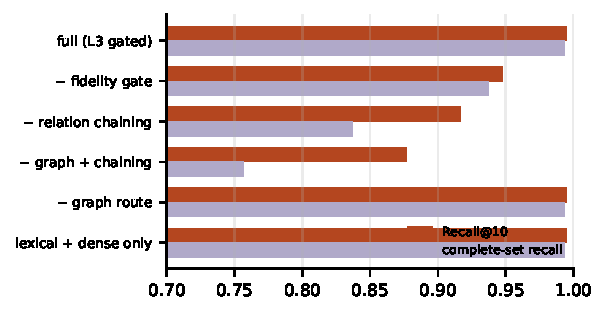
\includegraphics[width=\columnwidth]{fig_ablation.pdf}
\caption{Ablation on the synthetic benchmark ($n = 1\,000$, L3 gated, 3 seeds). Relation chaining carries the second hop; the gate carries the relation sentence through compression.}
\label{fig:ablation}
\end{figure}
One component removed at a time from the full system (Fig.~\ref{fig:ablation}). Relation chaining is the multi-hop component: without it Recall@10 falls from 0.995 to 0.917 and complete-set recall from 0.993 to 0.837; without the graph route as well, to 0.877 and 0.757. The gate protects relations as well as values: without it the gist drops the dependency sentence in 15\% of multi-hop cases, recall falls to 0.948 with triple the variance, and the retriever compensates with nearly three times as many raw expansions per query. Removing the trie route, the hub penalty or raw expansion changes recall by less than one point.

\section{Limitations}
\begin{enumerate}
\item \textbf{Re-implementations, not vendor code.} The six architecture baselines reproduce published retrieval designs with shared components; they are faithful to the architecture, not to the vendors' tuned systems.
\item \textbf{Paraphrase and regime results are single-seed and WordNet-based.} First-sense synonym substitution produces some unnatural rewrites, which is why even the dense route drops. Three seeds and an LLM-written paraphrase set are the obvious next step.
\item \textbf{LLM evaluation is limited.} 200 questions give $\pm 7$-point intervals; the accuracy differences among BM25 and the FidelityMem variants are not significant.
\item \textbf{One real dataset.} LongMemEval has a loader and a per-question runner in the repository; its results are not in this version.
\item \textbf{Compression on chat is small at $\rho = 0.95$.} Sessions carry a fact in nearly every sentence, so the gate backs off to raw. This is the bound being enforced on text with little to remove.
\item \textbf{Scale.} 10\,000 records in one process. Beyond about $10^5$ records the dense index and the controller's per-level recompression need an ANN index and sampled background optimisation.
\end{enumerate}

\section{Conclusion}
A memory system can be made to keep a stated share of its evidence recall, cheaply and without labels, by generating fidelity probes from the raw source and by searching policies under that bound with an out-of-sample gate. On a controlled synthetic protocol the resulting system dominates six current memory architectures on recall and evidence completeness while halving stored and served tokens. On real conversation data it does not beat BM25, and we show why: the benchmark's questions reuse the evidence's words. The system's value there is the controller, which selects lexical-only retrieval when the query log is literal and lexical+dense when it is paraphrased, matching the best fixed configuration in each regime without seeing the test questions. The unique parts are the gate, the controller and LLM-free ingestion; the rest is a careful integration of known components, released as an open package with the full evaluation stack.

\begin{thebibliography}{00}
\bibitem{facts} ``Facts as first-class objects: Knowledge objects for persistent LLM memory,'' arXiv:2603.17781, 2026.
\bibitem{fidelity} ``Fidelity before structure: Verbatim chunks beat lossy artifact extraction in long-conversation LLM memory,'' arXiv:2601.00821, 2026.
\bibitem{factwash} ``FACTWASH: Catching AI rewrites that wash hearsay into fact,'' arXiv:2608.03372, 2026.
\bibitem{memgpt} C. Packer et al., ``MemGPT: Towards LLMs as operating systems,'' arXiv:2310.08560, 2023.
\bibitem{hipporag} B. Guti\'errez et al., ``HippoRAG: Neurobiologically inspired long-term memory for large language models,'' arXiv:2405.14831, 2024.
\bibitem{zep} Zep / Graphiti, temporal knowledge graph memory, product documentation, 2025--2026.
\bibitem{mem0} Mem0, memory layer for AI agents, product documentation and benchmark pages, 2025--2026.
\bibitem{amem} ``A-MEM: Agentic memory for LLM agents,'' 2025.
\bibitem{r3mem} X. Wang et al., ``R$^3$Mem: Bridging memory retention and retrieval via reversible compression,'' in \emph{Findings of ACL}, 2025.
\bibitem{evolvemem} Y. Liu et al., ``EvolveMem: Self-evolving memory architecture via AutoResearch for LLM agents,'' arXiv:2605.13941, 2026.
\bibitem{memrl} Z. Zhang et al., ``MemRL: Self-evolving agents via runtime reinforcement learning on episodic memory,'' arXiv:2601.03192, 2026.
\bibitem{crystalmem} Y. Wu and J. Huang, ``CrystalMem,'' arXiv:2608.00303, 2026.
\bibitem{arc} T. Dang et al., ``Addressable recall compaction for long context-window control in AI agents,'' arXiv:2607.25066, 2026.
\bibitem{memrefine} S. Kim et al., ``MemRefine,'' arXiv:2606.13177, 2026.
\bibitem{ratedist} A. Colaco and M. Lahjouji, ``What to keep, what to forget: A rate--distortion view of memory compaction,'' arXiv:2607.08032, 2026.
\bibitem{tfusion} ``Training-free lexical-dense fusion for conversational-memory retrieval,'' arXiv:2606.04194, 2026.
\bibitem{fairness} ``Evidence-unit fairness and the limits of query-adaptive sparse-dense fusion in financial document retrieval,'' arXiv:2608.00183, 2026.
\bibitem{wrrf} ``Optimal fusion weights form intervals, not points: A latency-aware study of query-adaptive WRRF,'' arXiv:2610.24341, 2026.
\bibitem{vstash} J. Steffens, ``vstash: Local-first hybrid retrieval with adaptive fusion for LLM agents,'' arXiv:2604.15484, 2026.
\bibitem{locomo} A. Maharana et al., ``Evaluating very long-term conversational memory of LLM agents,'' in \emph{Proc. ACL}, 2024.
\end{thebibliography}

\end{document}
